\section{Aber ist Jutta Schell denn auch JS? Und bei Lufthansa?}
Aber ist Jutta Schell denn auch JS? Und bei Lufthansa?
Seit 1999 ist Jutta Schell laut eigenen Angaben mit Unterbrechungen für die Lufthansa tätig, seit 2016 als „Senior Manager Aviation Security“ \autocite{14}.\\

Und JS? Es lohnt ein Blick in den Chatverlauf der Gruppe DEMOKRATENCHAT, dann findet man heraus, dass JS Juristin ist (siehe \cref{image:13,image:14,image:15}).

\begin{figure}[hbt!]\centering
  \subfloat[\autocite{15}]{
    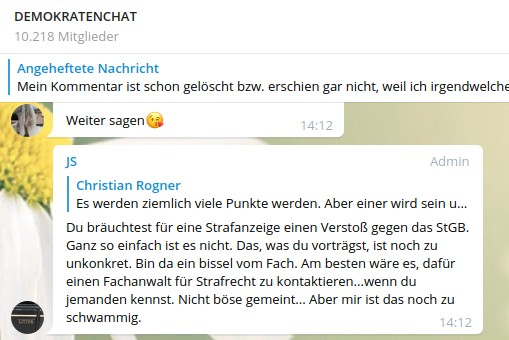
\includegraphics[width=0.3\textwidth]{images/image--013.jpg}
    \label{image:13}
  }
  \subfloat[\autocite{16}]{
    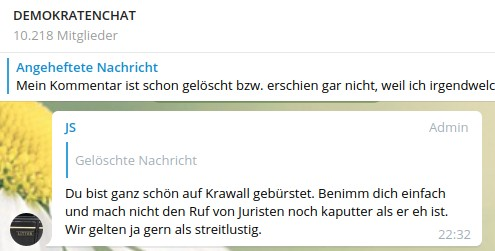
\includegraphics[width=.3\textwidth]{images/image--014.jpg}
    \label{image:14}
  }
  \subfloat[\autocite{17}]{
    
\includegraphics[width=.3\textwidth]{images/image--015.jpg}
    \label{image:15}
  }
  \caption{}
\end{figure}

Und die Frage, ob JS bei der Lufthansa ist? Ja, auch die beantwortet
sie uns selbst (siehe \cref{image:16}).
\begin{figure}[hbt!]\centering
  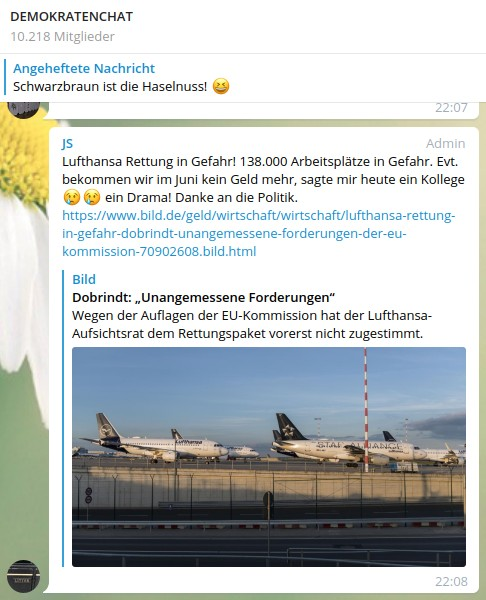
\includegraphics[width=0.4\textwidth]{images/image--016.jpg}
  \caption{\autocite{18}}\label{image:16}
\end{figure}

Die Frage ist jetzt: was machen wir daraus. Was macht die Deutsche
Lufthansa AG?\\

Als Luftfahrtunternehmen unterliegt die Lufthansa einer besonderen
Sorgfaltspflicht. Wir sind uns sicher, dass sich die Lufthansa AG
dieser großen Verantwortung voll bewusst ist, die Lufthansa, die als
Noch-DAX-Unternehmen gerade Staatshilfen erhält. Und es ist ja
auch gesetzlich geregelt, wie mit dieser Verantwortung umzugehen
ist.
\begin{quote}
  „In der Regel fehlt es an der erforderlichen Zuverlässigkeit,\newline
  [...]\newline
  3. wenn tatsächliche Anhaltspunkte dafür bestehen, dass die betroffene Person Bestrebungen nach § 3 Absatz 1 des Bundesverfassungsschutzgesetzes verfolgt oder unterstützt oder in den letzten zehn Jahren verfolgt oder unterstützt hat.“
\end{quote}
So steht es im Luftsicherheitsgesetz, Paragraph 7 Abs. 1a Satz 3\autocite{19}, dem Paragraphen, in dem es um die „Zuverlässigkeitsüberprüfungen“ geht. Und der hier erwähnte §3 Absatz 1 BVerfSchG – nun, da geht es unter anderem um

\begin{quote}
  „Bestrebungen, die gegen die freiheitliche demokratische Grundordnung, den Bestand oder die Sicherheit des Bundes oder eines Landes gerichtet sind oder eine ungesetzliche Beeinträchtigung der Amtsführung der Verfassungsorgane des Bundes oder eines Landes oder ihrer Mitglieder zum Ziele haben“\autocite{20}
\end{quote}
Sicher ist vieles in diesem Chat des Attila Hildmann vom Recht auf freie Meinungsäußerung gedeckt. Anonymous hält das Grundrecht auf freie Meinungsäußerung hoch. Aber vielleicht, liebe Deutsche Lufthansa AG, ist nicht alles, was frei geäußert wird, auch geeignet, Vertrauenaufrechtzuerhalten. Wenn Mitarbeiter aus dem Sicherheitsbereich mutmaßlich ihre Arbeitsrechner und Software verwenden, um Chatregeln für einen Telegram-Kanal von Attila Hildmann zu verfassen, wird es eng und darf auch überprüft werden, zuverlässigkeitsüberprüft sozusagen. Ach ja, und bevor es untergeht: sie erwähnte Event 201, bei dem auch Vertreter der Lufthansa waren \autocite{21} \autocite{22}.

\newpage
Attila Hildmann hat dazu einige Grafiken in der von Frau Schell in den Chatregeln verlinkten Dropbox \autocite{23}
hinterlegt\dots und meint daraus ableiten zu können, dass die Gates Foundation und andere Player – unter anderem Herr Knuchel von der Deutsche Lufthansa AG – die Corona Pandemie geübt und dann ausgeführt haben. Frau Schell und andere im DEMOKRATENCHAT sind davon wohl überzeugt. \\

Nun. Denn.
